\documentclass[]{article}
\usepackage{lmodern}
\usepackage{amssymb,amsmath}
\usepackage{ifxetex,ifluatex}
\usepackage{fixltx2e} % provides \textsubscript
\ifnum 0\ifxetex 1\fi\ifluatex 1\fi=0 % if pdftex
  \usepackage[T1]{fontenc}
  \usepackage[utf8]{inputenc}
\else % if luatex or xelatex
  \ifxetex
    \usepackage{mathspec}
  \else
    \usepackage{fontspec}
  \fi
  \defaultfontfeatures{Ligatures=TeX,Scale=MatchLowercase}
\fi
% use upquote if available, for straight quotes in verbatim environments
\IfFileExists{upquote.sty}{\usepackage{upquote}}{}
% use microtype if available
\IfFileExists{microtype.sty}{%
\usepackage{microtype}
\UseMicrotypeSet[protrusion]{basicmath} % disable protrusion for tt fonts
}{}
\usepackage[margin=1in]{geometry}
\usepackage{hyperref}
\hypersetup{unicode=true,
            pdfborder={0 0 0},
            breaklinks=true}
\urlstyle{same}  % don't use monospace font for urls
\usepackage{color}
\usepackage{fancyvrb}
\newcommand{\VerbBar}{|}
\newcommand{\VERB}{\Verb[commandchars=\\\{\}]}
\DefineVerbatimEnvironment{Highlighting}{Verbatim}{commandchars=\\\{\}}
% Add ',fontsize=\small' for more characters per line
\usepackage{framed}
\definecolor{shadecolor}{RGB}{248,248,248}
\newenvironment{Shaded}{\begin{snugshade}}{\end{snugshade}}
\newcommand{\KeywordTok}[1]{\textcolor[rgb]{0.13,0.29,0.53}{\textbf{#1}}}
\newcommand{\DataTypeTok}[1]{\textcolor[rgb]{0.13,0.29,0.53}{#1}}
\newcommand{\DecValTok}[1]{\textcolor[rgb]{0.00,0.00,0.81}{#1}}
\newcommand{\BaseNTok}[1]{\textcolor[rgb]{0.00,0.00,0.81}{#1}}
\newcommand{\FloatTok}[1]{\textcolor[rgb]{0.00,0.00,0.81}{#1}}
\newcommand{\ConstantTok}[1]{\textcolor[rgb]{0.00,0.00,0.00}{#1}}
\newcommand{\CharTok}[1]{\textcolor[rgb]{0.31,0.60,0.02}{#1}}
\newcommand{\SpecialCharTok}[1]{\textcolor[rgb]{0.00,0.00,0.00}{#1}}
\newcommand{\StringTok}[1]{\textcolor[rgb]{0.31,0.60,0.02}{#1}}
\newcommand{\VerbatimStringTok}[1]{\textcolor[rgb]{0.31,0.60,0.02}{#1}}
\newcommand{\SpecialStringTok}[1]{\textcolor[rgb]{0.31,0.60,0.02}{#1}}
\newcommand{\ImportTok}[1]{#1}
\newcommand{\CommentTok}[1]{\textcolor[rgb]{0.56,0.35,0.01}{\textit{#1}}}
\newcommand{\DocumentationTok}[1]{\textcolor[rgb]{0.56,0.35,0.01}{\textbf{\textit{#1}}}}
\newcommand{\AnnotationTok}[1]{\textcolor[rgb]{0.56,0.35,0.01}{\textbf{\textit{#1}}}}
\newcommand{\CommentVarTok}[1]{\textcolor[rgb]{0.56,0.35,0.01}{\textbf{\textit{#1}}}}
\newcommand{\OtherTok}[1]{\textcolor[rgb]{0.56,0.35,0.01}{#1}}
\newcommand{\FunctionTok}[1]{\textcolor[rgb]{0.00,0.00,0.00}{#1}}
\newcommand{\VariableTok}[1]{\textcolor[rgb]{0.00,0.00,0.00}{#1}}
\newcommand{\ControlFlowTok}[1]{\textcolor[rgb]{0.13,0.29,0.53}{\textbf{#1}}}
\newcommand{\OperatorTok}[1]{\textcolor[rgb]{0.81,0.36,0.00}{\textbf{#1}}}
\newcommand{\BuiltInTok}[1]{#1}
\newcommand{\ExtensionTok}[1]{#1}
\newcommand{\PreprocessorTok}[1]{\textcolor[rgb]{0.56,0.35,0.01}{\textit{#1}}}
\newcommand{\AttributeTok}[1]{\textcolor[rgb]{0.77,0.63,0.00}{#1}}
\newcommand{\RegionMarkerTok}[1]{#1}
\newcommand{\InformationTok}[1]{\textcolor[rgb]{0.56,0.35,0.01}{\textbf{\textit{#1}}}}
\newcommand{\WarningTok}[1]{\textcolor[rgb]{0.56,0.35,0.01}{\textbf{\textit{#1}}}}
\newcommand{\AlertTok}[1]{\textcolor[rgb]{0.94,0.16,0.16}{#1}}
\newcommand{\ErrorTok}[1]{\textcolor[rgb]{0.64,0.00,0.00}{\textbf{#1}}}
\newcommand{\NormalTok}[1]{#1}
\usepackage{graphicx,grffile}
\makeatletter
\def\maxwidth{\ifdim\Gin@nat@width>\linewidth\linewidth\else\Gin@nat@width\fi}
\def\maxheight{\ifdim\Gin@nat@height>\textheight\textheight\else\Gin@nat@height\fi}
\makeatother
% Scale images if necessary, so that they will not overflow the page
% margins by default, and it is still possible to overwrite the defaults
% using explicit options in \includegraphics[width, height, ...]{}
\setkeys{Gin}{width=\maxwidth,height=\maxheight,keepaspectratio}
\IfFileExists{parskip.sty}{%
\usepackage{parskip}
}{% else
\setlength{\parindent}{0pt}
\setlength{\parskip}{6pt plus 2pt minus 1pt}
}
\setlength{\emergencystretch}{3em}  % prevent overfull lines
\providecommand{\tightlist}{%
  \setlength{\itemsep}{0pt}\setlength{\parskip}{0pt}}
\setcounter{secnumdepth}{0}
% Redefines (sub)paragraphs to behave more like sections
\ifx\paragraph\undefined\else
\let\oldparagraph\paragraph
\renewcommand{\paragraph}[1]{\oldparagraph{#1}\mbox{}}
\fi
\ifx\subparagraph\undefined\else
\let\oldsubparagraph\subparagraph
\renewcommand{\subparagraph}[1]{\oldsubparagraph{#1}\mbox{}}
\fi

%%% Use protect on footnotes to avoid problems with footnotes in titles
\let\rmarkdownfootnote\footnote%
\def\footnote{\protect\rmarkdownfootnote}

%%% Change title format to be more compact
\usepackage{titling}

% Create subtitle command for use in maketitle
\newcommand{\subtitle}[1]{
  \posttitle{
    \begin{center}\large#1\end{center}
    }
}

\setlength{\droptitle}{-2em}
  \title{}
  \pretitle{\vspace{\droptitle}}
  \posttitle{}
  \author{}
  \preauthor{}\postauthor{}
  \date{}
  \predate{}\postdate{}


\begin{document}

\section{MultiVarSel}\label{multivarsel}

This is an R package to perform variable selection in the multivariate
linear model taking into account the dependence that may exist between
the responses. It consists in estimating beforehand the covariance
matrix \(\Sigma\) of the responses and to plug this estimator in a Lasso
criterion, in order to obtain a sparse estimator of the coefficient
matrix.

\subsection{Introduction and
Installation}\label{introduction-and-installation}

This vignette explains how to use the package \textbf{MultiVarSel} which
is dedicated to the variable selection in high-dimensional linear models
taking into account the dependence that may exist between the columns of
the observations matrix. The model can be described as follows :

\begin{equation}\label{eq:model}
Y=XB+E,
\end{equation}

where \(Y\) is a \(n\times q\) matrix of responses, \(X\) is a
\(n \times p\) matrix of covariables, \(B\) is a \(p\times q\) sparse
matrix of coefficients and \(E\) is a random error matrix such that
\(\forall i \in \{1,\cdots,n\}\),
\(E_i = (E_{i,1},\dots,E_{i,q})\sim\mathcal{N}(0,\Sigma)\). The package
consists in estimating \(\Sigma\) beforehand and to plug this estimator
in a Lasso criterion, in order to obtain a sparse estimator of the
coefficient matrix \(B\).

The package has to be installed and then loaded as follows :

\begin{Shaded}
\begin{Highlighting}[]
\CommentTok{# devtools::install_github("Marie-PerrotDockes/MultiVarSel")}
\KeywordTok{library}\NormalTok{(MultiVarSel)}
\end{Highlighting}
\end{Shaded}

\begin{verbatim}
## Loading required package: glmnet
\end{verbatim}

\begin{verbatim}
## Loading required package: Matrix
\end{verbatim}

\begin{verbatim}
## Loading required package: foreach
\end{verbatim}

\begin{verbatim}
## Loaded glmnet 2.0-16
\end{verbatim}

\begin{verbatim}
## Loading required package: parallel
\end{verbatim}

\begin{verbatim}
## Loading required package: tidyverse
\end{verbatim}

\begin{verbatim}
## -- Attaching packages ---------------------------------------------- tidyverse 1.2.1 --
\end{verbatim}

\begin{verbatim}
## √ ggplot2 2.2.1     √ purrr   0.2.4
## √ tibble  1.4.2     √ dplyr   0.7.4
## √ tidyr   0.8.0     √ stringr 1.3.0
## √ readr   1.1.1     √ forcats 0.3.0
\end{verbatim}

\begin{verbatim}
## -- Conflicts ------------------------------------------------- tidyverse_conflicts() --
## x purrr::accumulate() masks foreach::accumulate()
## x tidyr::expand()     masks Matrix::expand()
## x dplyr::filter()     masks stats::filter()
## x dplyr::lag()        masks stats::lag()
## x purrr::when()       masks foreach::when()
\end{verbatim}

\subsection{Numerical experiment}\label{numerical-experiment}

We first show an application of our methodology to a simulated data set
where the covariance matrix \(\Sigma\) is the covariance matrix of an
AR(1) process. We start by generating a random error matrix \(E\) as
described in the Introduction as follows.

\begin{Shaded}
\begin{Highlighting}[]
\NormalTok{n <-}\StringTok{ }\DecValTok{30}
\NormalTok{q <-}\StringTok{ }\DecValTok{100}
\NormalTok{p <-}\StringTok{ }\DecValTok{5}
\NormalTok{rho <-}\StringTok{ }\FloatTok{0.9}
\NormalTok{sparsity <-}\StringTok{ }\FloatTok{0.01}

\NormalTok{E <-}\StringTok{ }\KeywordTok{t}\NormalTok{(}\KeywordTok{sapply}\NormalTok{(}\DecValTok{1}\OperatorTok{:}\NormalTok{n,}\ControlFlowTok{function}\NormalTok{(i)\{}
  \KeywordTok{as.numeric}\NormalTok{(}\KeywordTok{arima.sim}\NormalTok{(q,}\DataTypeTok{model=}\KeywordTok{list}\NormalTok{(}\DataTypeTok{ar =}\NormalTok{ rho, }\DataTypeTok{ma =} \DecValTok{0}\NormalTok{)))}
\NormalTok{\}))}
\end{Highlighting}
\end{Shaded}

We then generate a sparse matrix \(B\) of coefficients and a matrix of
covariables \(X\).

\begin{Shaded}
\begin{Highlighting}[]
\NormalTok{s  <-}\StringTok{ }\KeywordTok{round}\NormalTok{(sparsity}\OperatorTok{*}\NormalTok{p}\OperatorTok{*}\NormalTok{q) }
\NormalTok{ij <-}\StringTok{ }\KeywordTok{arrayInd}\NormalTok{(}\KeywordTok{sample}\NormalTok{(}\DecValTok{1}\OperatorTok{:}\NormalTok{(p}\OperatorTok{*}\NormalTok{q), }\DataTypeTok{size =}\NormalTok{ s), }\KeywordTok{c}\NormalTok{(p,q))}
\NormalTok{B <-}\StringTok{ }\KeywordTok{sparseMatrix}\NormalTok{(}\DataTypeTok{i =}\NormalTok{ ij[, }\DecValTok{1}\NormalTok{], }\DataTypeTok{j =}\NormalTok{ ij[, }\DecValTok{2}\NormalTok{],}
                   \DataTypeTok{x =} \KeywordTok{runif}\NormalTok{(s) }\OperatorTok{*}\StringTok{ }\KeywordTok{sample}\NormalTok{(}\KeywordTok{c}\NormalTok{(}\OperatorTok{-}\DecValTok{1}\NormalTok{,}\DecValTok{1}\NormalTok{),s,}\DataTypeTok{rep=}\NormalTok{T),}
                   \DataTypeTok{dims =} \KeywordTok{c}\NormalTok{(p,q))}

\NormalTok{X <-}\StringTok{ }\KeywordTok{matrix}\NormalTok{(}\KeywordTok{rnorm}\NormalTok{(n}\OperatorTok{*}\NormalTok{p),n,p)}
   
\NormalTok{Y <-}\StringTok{ }\NormalTok{X }\OperatorTok\StringTok{ }\NormalTok{B  }\OperatorTok{+}\StringTok{ }\NormalTok{E}
\end{Highlighting}
\end{Shaded}

To apply our methodology we start by estimating the matrix \(E\) by
computing the residuals independently on all the columns of \(Y\):

\begin{Shaded}
\begin{Highlighting}[]
\NormalTok{residual <-}\StringTok{ }\KeywordTok{lm}\NormalTok{(}\KeywordTok{as.matrix}\NormalTok{(Y) }\OperatorTok{~}\StringTok{ }\NormalTok{X }\OperatorTok{-}\StringTok{ }\DecValTok{1}\NormalTok{)}\OperatorTok{$}\NormalTok{residuals}
\end{Highlighting}
\end{Shaded}

We then use a Portmanteau test to check if each row of this matrix
\(\widehat{E}\) is a white noise or not.

\begin{Shaded}
\begin{Highlighting}[]
\KeywordTok{whitening_test}\NormalTok{(residual)}
\end{Highlighting}
\end{Shaded}

\begin{verbatim}
## [1] 0
\end{verbatim}

The \(p-value\) is really small hence we reject the hypothesis that each
row of the residual matrix is a white noise which is an expected result
since each row of \(E\) is an AR(1) process.

We then try to remove the dependence among the columns of the residuals
matrix by estimating the covariance matrix of the rows of \(E\). To
estimate it we try different structures for this covariance. The
simplest assumption is that each row of \(E\) follows an \(AR(1)\)
process, we also propose a modelisation where each row is an
\(ARMA(p,q)\) process and a nonparametric one where \(\Sigma\) is only
assumed to be Toeplitz. To compare this different estimations we perform
a Portmenteau test on the ``whithened'' matrix
\(\widehat{E}\widehat{\Sigma}^{-1/2}\), where \(\hat{\Sigma^{-1/2}}\) is
the square root of the inverse of the estimation of \(\Sigma\).

With the following code we test the AR(1), ARMA(1,1) and nonparametric
dependence structures :

\begin{Shaded}
\begin{Highlighting}[]
\NormalTok{result <-}\StringTok{ }\KeywordTok{whitening_choice}\NormalTok{(residual, }\KeywordTok{c}\NormalTok{(}\StringTok{"AR1"}\NormalTok{,}\StringTok{"ARMA"}\NormalTok{,}\StringTok{"nonparam"}\NormalTok{), }\DataTypeTok{pAR =} \DecValTok{1}\NormalTok{, }\DataTypeTok{qMA =} \DecValTok{1}\NormalTok{)}
\NormalTok{result}
\end{Highlighting}
\end{Shaded}

\begin{verbatim}
##          Pvalue    Decision
## AR1       0.883 WHITE NOISE
## ARMA 1 1  0.921 WHITE NOISE
## nonparam  0.991 WHITE NOISE
\end{verbatim}

We then select the simplest model that allows us to remove the
dependence in the data, in that case the \(AR(1)\) modelling. We compute
the square root of the inverse of the estimator of the covariance matrix
of each row of the residuals matrix using the \(AR(1)\) modelling as
follows:

\begin{Shaded}
\begin{Highlighting}[]
\NormalTok{square_root_inv_hat_Sigma <-}\StringTok{ }\KeywordTok{whitening}\NormalTok{(residual, }\StringTok{"AR1"}\NormalTok{, }\DataTypeTok{pAR =} \DecValTok{1}\NormalTok{, }\DataTypeTok{qMA =} \DecValTok{0}\NormalTok{)}
\end{Highlighting}
\end{Shaded}

In order to whiten the data (remove the dependence), we transform the
data as follows:

\begin{equation}\label{eq:model_whitened}
\boldsymbol{Y}\widehat{\boldsymbol{\Sigma}}_q^{-1/2}  
    =\boldsymbol{X}\boldsymbol{B}\widehat{\boldsymbol{\Sigma}}_q^{-1/2} + \boldsymbol{E}\widehat{\boldsymbol{\Sigma}}_q^{-1/2}.
\end{equation}

The idea is then to use the Lasso criterion introduced by Tibshirani in
1996, and available in the R package \texttt{glmnet} on these whitened
data. We recall that in the classical linear model
\[{\mathcal{Y}}={\mathcal{X}}\mathcal{B}+{\mathcal{E}},\] where
\(\mathcal{Y}\), \(\mathcal{B}\) and \(\mathcal{E}\) are vectors and
\(\mathcal{X}\) is a matrix, the Lasso estimator of \(\mathcal{B}\) is
defined by

\begin{equation*}
      \widehat{\mathcal{B}}(\lambda)=\textrm{Argmin}_\mathcal{B}\left\{\|\mathcal{Y}-\mathcal{X}\mathcal{B}\|_2^2+\lambda\|\mathcal{B}\|_1\right\}.
    \end{equation*}

In order to be able to use the Lasso criterion we will apply the vec
operator to \eqref{eq:model_whitened}

\begin{align*}
      {\mathcal{Y}}&=
                     vec(\boldsymbol{Y}\widehat{\boldsymbol{\Sigma}}_q^{-1/2})  
=vec(\boldsymbol{X}\boldsymbol{B}\widehat{\boldsymbol{\Sigma}}_q^{-1/2})
                     +vec(\boldsymbol{E}\widehat{\boldsymbol{\Sigma}}_q^{-1/2})\\
                   &=\textcolor{blue}{((\widehat{\boldsymbol{\Sigma}}_q^{-1/2})'\otimes \boldsymbol{X})}\textcolor{green}{vec(\boldsymbol{B})}
                     +\textcolor{red}{vec(\boldsymbol{E}\widehat{\boldsymbol{\Sigma}}_q^{-1/2})}\\
                   &=\textcolor{blue}{\mathcal{X}}\textcolor{green}{\mathcal{B}}+\textcolor{red}{\mathcal{E}}.
    \end{align*}

The Lasso criterion applied to
\(\mathcal{Y}}=vec(\boldsymbol{Y}\widehat{\boldsymbol{\Sigma}}_q^{-1/2})\)
will provide an estimation of the non null positions of
\(\mathcal{B}=vec(\boldsymbol{B})\) and hence the non null positions of
\(B\). In order to avoid false positive positions we add a stability
selection step. These different steps (whitening, vectorization, Lasso,
stability selection) are implemented in the function
\texttt{variable_selection} of the R package \texttt{MultiVarSel}.

\begin{Shaded}
\begin{Highlighting}[]
\NormalTok{Frequencies=}\KeywordTok{variable_selection}\NormalTok{(}\DataTypeTok{Y =}\NormalTok{ Y, }\DataTypeTok{X =}\NormalTok{ X, }\DataTypeTok{nb_repli =} \DecValTok{50}\NormalTok{, }\DataTypeTok{typeDep =}  \StringTok{"AR1"}\NormalTok{)}
\end{Highlighting}
\end{Shaded}

In the previous command line, \texttt{nb_repli} corresponds to the
number of replications which is used in the stability selection. Here it
is equal to 50 but in practice we recommend to take it equal to 1000.
The following plot displays the frequencies at which each coefficient of
\(B\) is considered as being non null.

\begin{Shaded}
\begin{Highlighting}[]
\NormalTok{p <-}\StringTok{ }\KeywordTok{ggplot}\NormalTok{(}\DataTypeTok{data =}\NormalTok{ Frequencies[Frequencies}\OperatorTok{$}\NormalTok{Frequencies }\OperatorTok{>=}\StringTok{ }\FloatTok{0.95}\NormalTok{, ],}
           \KeywordTok{aes}\NormalTok{(}\DataTypeTok{x =}\NormalTok{ Names_of_Y, }\DataTypeTok{y =}\NormalTok{ Names_of_X, }\DataTypeTok{color =}\NormalTok{ Frequencies, }\DataTypeTok{fill =}\NormalTok{ Frequencies)) }\OperatorTok{+}
\StringTok{           }\KeywordTok{geom_tile}\NormalTok{(}\DataTypeTok{size =} \FloatTok{0.75}\NormalTok{) }\OperatorTok{+}\StringTok{ }\KeywordTok{scale_color_gradient2}\NormalTok{(}\DataTypeTok{midpoint =} \FloatTok{0.95}\NormalTok{, }\DataTypeTok{mid =} \StringTok{'orange'}\NormalTok{)  }\OperatorTok{+}\StringTok{ }\KeywordTok{scale_fill_gradient2}\NormalTok{(}\DataTypeTok{midpoint =} \FloatTok{0.95}\NormalTok{, }\DataTypeTok{mid =} \StringTok{'orange'}\NormalTok{) }\OperatorTok{+}
\StringTok{           }\KeywordTok{theme_bw}\NormalTok{() }\OperatorTok{+}\StringTok{ }\KeywordTok{ylab}\NormalTok{(}\StringTok{'Levels of X'}\NormalTok{) }\OperatorTok{+}\StringTok{ }\KeywordTok{xlab}\NormalTok{(}\StringTok{'Names of Y'}\NormalTok{)}
\NormalTok{p}
\end{Highlighting}
\end{Shaded}

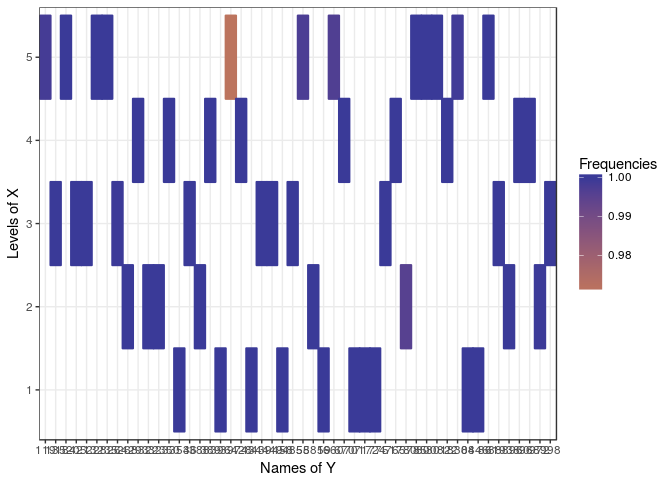
\includegraphics{README_files/figure-latex/unnamed-chunk-9-1.pdf}

If we take a threshold of 0.95, meaning that we keep as non null values
only the ones that are considered as non null in more than 95\% of the
times we have a True Positive Rate equal to 0.6 and a False Positive
Rate equal to 0.

\subsection{An exemple in
metabolomics}\label{an-exemple-in-metabolomics}

In this section we study a LC-MS (Liquid Chromatography-Mass
Spectrometry) data set made of African copals samples. The samples
correspond to ethanolic extracts of copals produced by trees belonging
to two genera Copaifera (C) and Trachylobium (T) with a second level of
classification coming from the geographical provenance of the Copaifera
samples (West (W) or East (E) Africa). Since all the Trachylobium
samples come from East Africa, we can use the modeling proposed in
\eqref{eq:model} where \(X\) is a one-way ANOVA design matrix with 3
levels. Our goal is to identify the most important features (the m/z
values) characterizing the different levels. In order to have a fast and
reproducible example we focus in this section on the 200 first
metabolites (\(q=200\)) but our package can handle much larger datasets
(up to \(q=5000\) in a few minutes).

\begin{Shaded}
\begin{Highlighting}[]
\KeywordTok{data}\NormalTok{(}\StringTok{"copals_camera"}\NormalTok{)}
\NormalTok{Y <-}\StringTok{ }\NormalTok{Y }\OperatorTok\StringTok{  }\KeywordTok{as.data.frame}\NormalTok{() }\OperatorTok\StringTok{ }\KeywordTok{select}\NormalTok{(}\DecValTok{1}\OperatorTok{:}\DecValTok{200}\NormalTok{) }\OperatorTok\StringTok{ }\KeywordTok{scale}\NormalTok{()}
\end{Highlighting}
\end{Shaded}

We build the design matrix as follows

\begin{Shaded}
\begin{Highlighting}[]
\NormalTok{X <-}\StringTok{ }\KeywordTok{model.matrix}\NormalTok{( }\OperatorTok{~}\StringTok{ }\NormalTok{group }\OperatorTok{+}\StringTok{ }\DecValTok{0}\NormalTok{)}
\end{Highlighting}
\end{Shaded}

We start by computing the residuals of the one-way ANOVA model for each
metabolite independently.

\begin{Shaded}
\begin{Highlighting}[]
\NormalTok{residuals=}\KeywordTok{lm}\NormalTok{(}\KeywordTok{as.matrix}\NormalTok{(Y) }\OperatorTok{~}\StringTok{ }\NormalTok{X }\OperatorTok{-}\StringTok{ }\DecValTok{1}\NormalTok{)}\OperatorTok{$}\NormalTok{residuals}
\end{Highlighting}
\end{Shaded}

Then we test if the columns of the residuals are independent using the
Portmanteau test.

\begin{Shaded}
\begin{Highlighting}[]
\KeywordTok{whitening_test}\NormalTok{(residuals)}
\end{Highlighting}
\end{Shaded}

\begin{verbatim}
## [1] 5.676735e-229
\end{verbatim}

The \(p-value\) is really small and thus the hypothesis that each row of
\(E\) is a white noise is rejected. We try our different covariance
modellings for the residuals and see if one manages to remove the
dependence among the columns of the residuals matrix by using a
Portmanteau test.

\begin{Shaded}
\begin{Highlighting}[]
\NormalTok{result=}\KeywordTok{whitening_choice}\NormalTok{(residuals, }\KeywordTok{c}\NormalTok{(}\StringTok{"AR1"}\NormalTok{, }\StringTok{"nonparam"}\NormalTok{, }\StringTok{"ARMA"}\NormalTok{), }\DataTypeTok{pAR =} \DecValTok{1}\NormalTok{, }\DataTypeTok{qMA =} \DecValTok{1}\NormalTok{)}
\NormalTok{result}
\end{Highlighting}
\end{Shaded}

\begin{verbatim}
##          Pvalue       Decision
## AR1           0 NO WHITE NOISE
## nonparam  0.992    WHITE NOISE
## ARMA 1 1  0.653    WHITE NOISE
\end{verbatim}

From this result, we observe that the \(AR(1)\) modelling does not
remove the dependence among the data but the two others do. We select
the \(ARMA(1,1)\) modelling which is simpler than the nonparametric one.

In this application, the design matrix \(X\) is the design matrix of a
one-way ANOVA. In that scenario we recommend to use the argument
\texttt{group =} ``your qualitative variable'' in the
\texttt{variable_selection} function. This argument will ensure that in
the cross-validation the different fold are homogeneously distributed
among the levels of the qualitative variable.

\begin{Shaded}
\begin{Highlighting}[]
\NormalTok{Frequencies <-}\StringTok{ }\KeywordTok{variable_selection}\NormalTok{(}\DataTypeTok{Y =}\NormalTok{ Y, }\DataTypeTok{group =}\NormalTok{ group, }\DataTypeTok{nb_repli =} \DecValTok{100}\NormalTok{, }\DataTypeTok{typeDep =} \StringTok{'ARMA'}\NormalTok{, }\DataTypeTok{pAR =} \DecValTok{1}\NormalTok{, }\DataTypeTok{qMA =} \DecValTok{1}\NormalTok{)}
\end{Highlighting}
\end{Shaded}

\begin{verbatim}
## Warning in arima(x, order = c(pAR, 0, qMA)): possible convergence problem:
## optim gave code = 1
\end{verbatim}

The following plot displays the frequencies at which each coefficient of
\(B\) is considered as being non null which corresponds to the features
(m/z values) characterizing the different levels.

\begin{Shaded}
\begin{Highlighting}[]
\NormalTok{Frequencies}\OperatorTok{$}\NormalTok{Names_of_Y <-}\StringTok{ }\KeywordTok{as.numeric}\NormalTok{(}\KeywordTok{gsub}\NormalTok{(}\StringTok{'X'}\NormalTok{,}\StringTok{''}\NormalTok{,Frequencies}\OperatorTok{$}\NormalTok{Names_of_Y))}
\NormalTok{p <-}\StringTok{ }\KeywordTok{ggplot}\NormalTok{(}\DataTypeTok{data =}\NormalTok{ Frequencies[Frequencies}\OperatorTok{$}\NormalTok{Frequencies }\OperatorTok{>=}\StringTok{ }\FloatTok{0.95}\NormalTok{, ],}
           \KeywordTok{aes}\NormalTok{(}\DataTypeTok{x =}\NormalTok{ Names_of_Y, }\DataTypeTok{y =}\NormalTok{ Names_of_X, }\DataTypeTok{color =}\NormalTok{ Frequencies, }\DataTypeTok{fill =}\NormalTok{ Frequencies)) }\OperatorTok{+}
\StringTok{           }\KeywordTok{geom_tile}\NormalTok{(}\DataTypeTok{size =} \FloatTok{0.75}\NormalTok{) }\OperatorTok{+}\StringTok{ }\KeywordTok{scale_color_gradient2}\NormalTok{(}\DataTypeTok{midpoint =} \FloatTok{0.95}\NormalTok{, }\DataTypeTok{mid =} \StringTok{'orange'}\NormalTok{)  }\OperatorTok{+}\StringTok{ }\KeywordTok{scale_fill_gradient2}\NormalTok{(}\DataTypeTok{midpoint =} \FloatTok{0.95}\NormalTok{, }\DataTypeTok{mid =} \StringTok{'orange'}\NormalTok{) }\OperatorTok{+}
\StringTok{           }\KeywordTok{theme_bw}\NormalTok{() }\OperatorTok{+}\StringTok{ }\KeywordTok{ylab}\NormalTok{(}\StringTok{'Levels of X'}\NormalTok{) }\OperatorTok{+}\StringTok{ }\KeywordTok{xlab}\NormalTok{(}\StringTok{'m/z'}\NormalTok{)}
\NormalTok{p}
\end{Highlighting}
\end{Shaded}

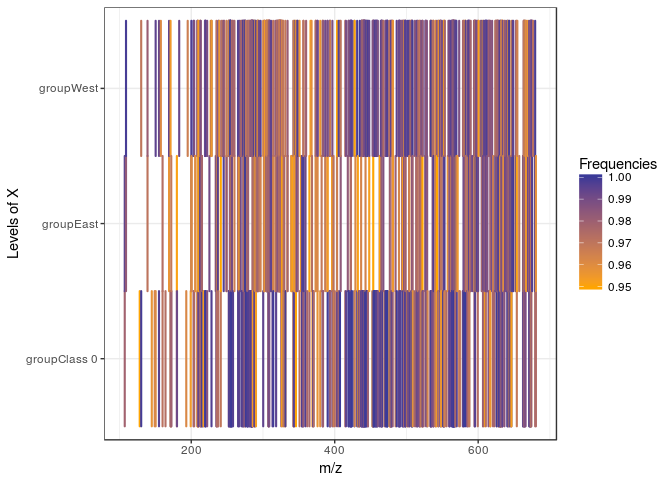
\includegraphics{README_files/figure-latex/unnamed-chunk-16-1.pdf}

Hereafter, we also provide some information about the R session

\begin{Shaded}
\begin{Highlighting}[]
 \KeywordTok{sessionInfo}\NormalTok{()}
\end{Highlighting}
\end{Shaded}

\begin{verbatim}
## R version 3.4.4 (2018-03-15)
## Platform: x86_64-pc-linux-gnu (64-bit)
## Running under: Ubuntu 16.04.4 LTS
## 
## Matrix products: default
## BLAS: /usr/lib/libblas/libblas.so.3.6.0
## LAPACK: /usr/lib/lapack/liblapack.so.3.6.0
## 
## locale:
##  [1] LC_CTYPE=fr_FR.UTF-8       LC_NUMERIC=C              
##  [3] LC_TIME=fr_FR.UTF-8        LC_COLLATE=fr_FR.UTF-8    
##  [5] LC_MONETARY=fr_FR.UTF-8    LC_MESSAGES=fr_FR.UTF-8   
##  [7] LC_PAPER=fr_FR.UTF-8       LC_NAME=C                 
##  [9] LC_ADDRESS=C               LC_TELEPHONE=C            
## [11] LC_MEASUREMENT=fr_FR.UTF-8 LC_IDENTIFICATION=C       
## 
## attached base packages:
## [1] parallel  stats     graphics  grDevices utils     datasets  methods  
## [8] base     
## 
## other attached packages:
##  [1] MultiVarSel_1.1.2 forcats_0.3.0     stringr_1.3.0    
##  [4] dplyr_0.7.4       purrr_0.2.4       readr_1.1.1      
##  [7] tidyr_0.8.0       tibble_1.4.2      ggplot2_2.2.1    
## [10] tidyverse_1.2.1   glmnet_2.0-16     foreach_1.4.4    
## [13] Matrix_1.2-13    
## 
## loaded via a namespace (and not attached):
##  [1] reshape2_1.4.3   haven_1.1.1      lattice_0.20-35  colorspace_1.3-2
##  [5] htmltools_0.3.6  yaml_2.1.18      rlang_0.2.0      pillar_1.2.1    
##  [9] foreign_0.8-69   glue_1.2.0       modelr_0.1.1     readxl_1.0.0    
## [13] bindrcpp_0.2     bindr_0.1        plyr_1.8.4       munsell_0.4.3   
## [17] gtable_0.2.0     cellranger_1.1.0 rvest_0.3.2      codetools_0.2-15
## [21] psych_1.8.3.3    evaluate_0.10.1  labeling_0.3     knitr_1.20      
## [25] broom_0.4.4      Rcpp_0.12.16     backports_1.1.2  scales_0.5.0    
## [29] jsonlite_1.5     mnormt_1.5-5     hms_0.4.2        digest_0.6.15   
## [33] stringi_1.1.7    grid_3.4.4       rprojroot_1.3-2  cli_1.0.0       
## [37] tools_3.4.4      magrittr_1.5     lazyeval_0.2.0   crayon_1.3.4    
## [41] pkgconfig_2.0.1  xml2_1.2.0.9000  lubridate_1.7.3  assertthat_0.2.0
## [45] rmarkdown_1.9    httr_1.3.1       rstudioapi_0.7   iterators_1.0.9 
## [49] R6_2.2.2         nlme_3.1-131.1   compiler_3.4.4
\end{verbatim}


\end{document}
